\subsection{Results of the unsupervised approach}

In this section, we assess the performance of the unsupervised approach with the evaluation sets. We first confirm the results of our qualitative assessment of the vector combination methods, which indicated that summing the vectors yields better results than averaging or concatenating them. The performance of the sum method on the venue and \acrshort{ddc} evaluation sets is considerably higher than that of the other two methods.

We then evaluate the performance of the sum method in the handwritten evaluation set. Its performance is lower than in the other evaluation sets, where only fields of study are considered. This is to be expected, given that there are 2,157 candidate subjects instead of 19, but it is still low.

We already discussed possible reasons for this difference in performance in section \ref{unsupervised_approach_conclusion}. The main challenge is the size of the dataset. The small amount of relationships that can be built between documents, and also between documents and venues, hinders the representations of the documents.

\subsubsection{Comparing the vector combination methods}

\begin{figure}
  \begin{subfigure}[t]{.45\textwidth}
    \centering
    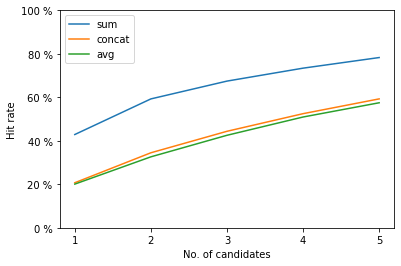
\includegraphics[width=\textwidth]{figures/unsupervised_approach/results/cosine_methods_ddc.png}
    \caption{DDC subjects}
    \label{fig:cosine_methods_ddc}
  \end{subfigure}
  \begin{subfigure}[t]{.45\textwidth}
    \centering
    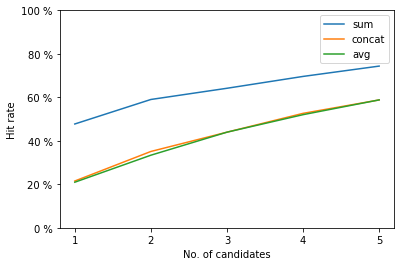
\includegraphics[width=\textwidth]{figures/unsupervised_approach/results/cosine_methods_venues.png}
    \caption{Venues}
    \label{fig:cosine_methods_venues}
  \end{subfigure}
  \caption{Hit rate of the three distance metrics in the evaluation sets.}
  \label{fig:combination_eval}
\end{figure}

We compare the three distance metrics on the two evaluation sets that consider fields, namely the \acrshort{ddc} and the venue evaluation sets. The hit rate of the combination methods is shown in figure \ref{fig:combination_eval}. The sum method outperforms the other two methods by a large margin in both datasets, the difference being usually over 20 \%. The other two methods behave similarly.

The sum method performs better for all considered numbers of candidates. It is also the most efficient, as all objects are represented by 100-dimensional vectors, as well as the only one that doesn't discard any information. The other two methods truncate word vectors, to match the sizes between the representations of documents and subjects.

\subsubsection{Results on the evaluation sets} \label{unsupervised_approach_results_eval}

\begin{figure}
  \begin{subfigure}[t]{.32\textwidth}
    \centering
    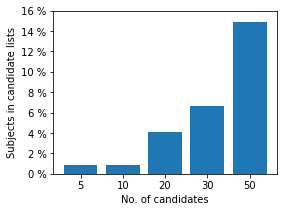
\includegraphics[width=\textwidth]{figures/unsupervised_approach/results/first_hw.png}
    \caption{Handwritten subjects}
    \label{fig:first_hw}
  \end{subfigure}
  \begin{subfigure}[t]{.32\textwidth}
    \centering
    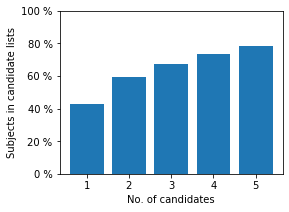
\includegraphics[width=\textwidth]{figures/unsupervised_approach/results/first_ddc.png}
    \caption{DDC subjects}
    \label{fig:first_ddc}
  \end{subfigure}
   \begin{subfigure}[t]{.32\textwidth}
    \centering
    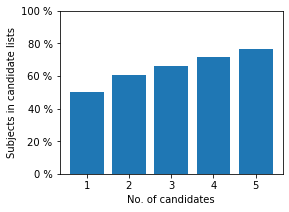
\includegraphics[width=\textwidth]{figures/unsupervised_approach/results/first_venue.png}
    \caption{Venues}
    \label{fig:first_venue}
  \end{subfigure}
  \caption{Hit rate of the unsupervised approach in the evaluation sets.}
  \label{fig:first_eval}
\end{figure}

Here we present the final results of the unsupervised approach, using the sum method as the distance metric. We have computed the distances between the documents and the subjects that descend from the five fields that are the closest to each document. We then store the 50 subjects that are the closest to each document. The hit rate of this approach on the evaluation set is depicted in figure \ref{fig:first_eval}. The hit rate on the \acrshort{ddc} and venue evaluation sets was already shown when comparing the different distance metrics.

The hit rate of this approach on the handwritten set is lower than in the other two datasets. Being accurate is much less likely in this set, as it has 2,157 options instead of 19, so the lower hit rate is to be expected. The hit rate of the model increases dramatically when more candidates are considered, reaching a maximum value of 15 \% when the 50 most similar subjects are considered. Recall that the subjects present in this evaluation set are not necessarily those that describe best the documents they are assigned to. They are merely those that appear in our subset of \acrshort{mag} subjects. Therefore, it is normal that the hit rate is so low when considering small numbers of candidates.

\begin{figure}
    \centering
    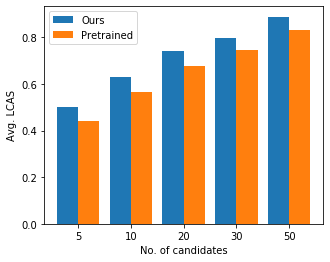
\includegraphics[width=.7\textwidth]{figures/unsupervised_approach/results/avg_lcas.png}
    \caption{Avg. LCAS of the unsupervised approach method, with and without pre-trained embeddings.}
    \label{fig:avg_lcas}
\end{figure}

\begin{figure}
    \centering
    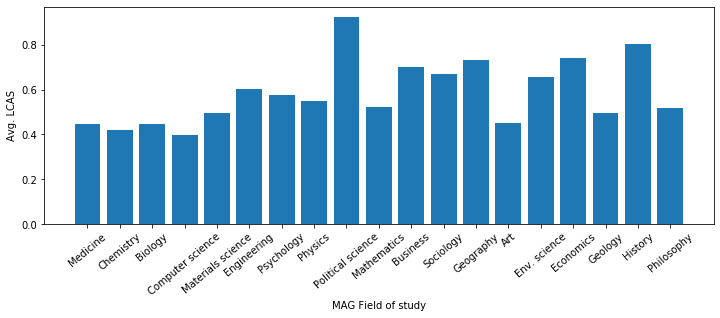
\includegraphics[width=\textwidth]{figures/unsupervised_approach/results/field_lcas.png}
    \caption{Avg. LCAS for each field using the unsupervised approach method and considering five candidates.}
    \label{fig:field_lcas}
\end{figure}

Regarding the \acrfull{lcas}, shown in figure \ref{fig:avg_lcas}, it steadily increases with the number of candidates, reaching a maximum average value of $0.89$. This value is very high, meaning that the guesses are close to the correct subjects in the subject hierarchy. We have also computed the average \acrshort{lcas} for each field, when considering five candidates. This is shown in figure \ref{fig:field_lcas}. \textit{Political Science} has a remarkably high value, over $0.9$, which results of averaging the \acrshort{lcas} of 898 assignments. Apparently, the model is accurately identifying the field.

On the other hand, \textit{Computer science} has a low average \acrshort{lcas} considering how popular the field is in our dataset. It may have to do with the fact that the subjects present in the handwritten set are not the top choices for the indexed documents and therefore do not appear in the top five candidates. When considering 50 candidates, \textit{Computer science} reaches an \acrshort{lcas} of $0.8$, and all other fields over $0.75$

\subsubsection{Using pre-trained embeddings} \label{unsupervised_approach_results_pretrained}

\begin{figure}
  \begin{subfigure}[t]{.32\textwidth}
    \centering
    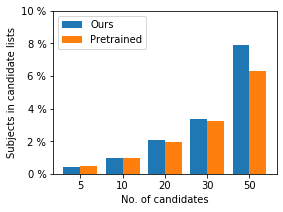
\includegraphics[width=\textwidth]{figures/unsupervised_approach/results/pretrained_hw.png}
    \caption{Handwritten subjects}
    \label{fig:pretrained_hw}
  \end{subfigure}
  \begin{subfigure}[t]{.32\textwidth}
    \centering
    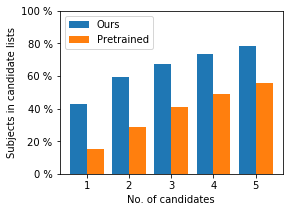
\includegraphics[width=\textwidth]{figures/unsupervised_approach/results/pretrained_ddc.png}
    \caption{DDC subjects}
    \label{fig:pretrained_ddc}
  \end{subfigure}
   \begin{subfigure}[t]{.32\textwidth}
    \centering
    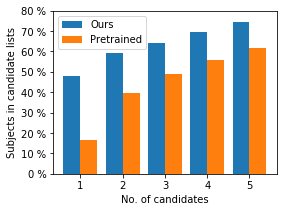
\includegraphics[width=\textwidth]{figures/unsupervised_approach/results/pretrained_venue.png}
    \caption{Venues}
    \label{fig:pretrained_venue}
  \end{subfigure}
  \caption{Hit rate of the unsupervised approach in the evaluation sets, with and without pre-trained embeddings.}
  \label{fig:pretrained_eval}
\end{figure}

Using pre-trained vector embeddings is common practice for \acrfull{nlp} tasks \cite{mikolov2017advances}. Such embeddings are trained on very large corpora and thus more accurately represent their corresponding words. Especially tasks on small datasets benefit from this transfer. However, technical datasets may not benefit as much from such pre-trained embeddings. They include words that are otherwise rare in non-scientific literature, and the style of writing is also different.

Here, we implement the same unsupervised approach, only changing the embeddings used to vectorize the texts. Instead of using the embeddings we have trained on our corpus, we use the pre-trained ones presented in section \ref{supervised_approach_embeddings}. Less than 3 \% of the words of our texts are not present in the file of pre-trained embeddings. If it were more, the lack of coverage would significantly hinder the performance of the method. This could still be the case, if the most distinctive words of each text are the ones missing.

Surprisingly, our own embeddings offer better results on the evaluation datasets, as shown in figure \ref{fig:pretrained_eval}. The method with our embeddings outperforms the one with the pre-trained embeddings on every dataset, for every number of candidates. Especially for the datasets regarding fields, the \acrshort{ddc} and venue datasets, the difference in hit rate is mostly around 30 to 50 \%. In the handwritten set, the difference is not so large, given that both models perform poorly.

This shows that our embeddings do a better job at representing the documents of the repositories. It is surprising that they are so much better, given the small size of our corpus. However, given how technical our corpus is, including fields both from the natural and the social sciences, it is to be expected that pre-trained embeddings don't work as well as in other use cases, where the data is similar to the one used to pre-train the embeddings.

The average \acrshort{lcas} of this method is depicted in figure \ref{fig:field_lcas} for several number of candidates. There it can be seen that using our own embeddings consistently improves the \acrshort{lcas} by $0.1$, which is a significant difference. Still, this method reaches an avg. \acrshort{lcas} of $0.8$ when considering 50 candidates.
